% 2007 年湖北卷理科第 18 题：三棱锥 V-ABC，VC⊥底面 ABC，AC⊥BC，
%   D 为 AB 的中点，∠VDC=θ。
% 来源 PDF：gaokaomath-src/普通高考/2007/2007湖北理.pdf
% SHA-256：e767bc35f619e1cd5a96990bd14ba9415b3a440d7d9f5766e43aa6433844b65d
% 原页：2007湖北理.pdf 第 2 页（A3 三栏）第 1 栏，书页码 376。
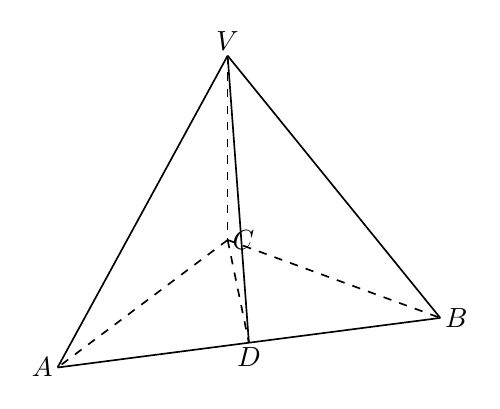
\begin{tikzpicture}[scale=0.9, semithick,
  every node/.style={inner sep=1.5pt}]
  \coordinate (V) at (3.0,5.0);
  \coordinate (C) at (3.0,2.4);
  \coordinate (A) at (0.6,0.6);
  \coordinate (B) at (6.0,1.3);
  \coordinate (D) at (3.3,0.95);

  \draw (V) -- (A);
  \draw (V) -- (B);
  \draw (V) -- (D);
  \draw (A) -- (B);
  \draw[dashed] (V) -- (C);
  \draw[dashed] (C) -- (A);
  \draw[dashed] (C) -- (B);
  \draw[dashed] (C) -- (D);

  \node[above] at (V) {$V$};
  \node[right] at (C) {$C$};
  \node[left] at (A) {$A$};
  \node[right] at (B) {$B$};
  \node[below] at (D) {$D$};
\end{tikzpicture}
